\documentclass{beamer}

\mode<presentation>
{
  \usetheme{Warsaw}

  \setbeamercovered{transparent}
}


\usepackage[english]{babel}

\usepackage[latin1]{inputenc}

\usepackage[T1]{fontenc}

% for code listings
\usepackage{listings}
\lstset
{
    language=[LaTeX]TeX,
    breaklines=true,
    keywordstyle=\color{blue},
    identifierstyle=\color{magenta},
	commentstyle=\color{purple},
    basicstyle=\tt\large,
	frame=single,
}

% for flowcharts
\usepackage{tikz}
\usetikzlibrary{shapes.geometric, arrows}


\title{Introduction to \LaTeX\ Workshop}

\author[HKN] % (optional, use only with lots of authors)
{By HKN}
% - Use the \inst{?} command only if the authors have different
%   affiliation.

\date[Short Occasion] % (optional)
{\today}

% This is only inserted into the PDF information catalog. Can be left
% out. 

% If you have a file called "university-logo-filename.xxx", where xxx
% is a graphic format that can be processed by latex or pdflatex,
% resp., then you can add a logo as follows:

% \pgfdeclareimage[height=0.5cm]{university-logo}{university-logo-filename}
% \logo{\pgfuseimage{university-logo}}


% If you wish to uncover everything in a step-wise fashion, uncomment
% the following command: 

%\beamerdefaultoverlayspecification{<+->}

\begin{document}

\begin{frame}
  \titlepage
\end{frame}

\begin{frame}{Outline}
  \tableofcontents
  % You might wish to add the option [pausesections]
\end{frame}


% Since this a solution template for a generic talk, very little can
% be said about how it should be structured. However, the talk length
% of between 15min and 45min and the theme suggest that you stick to
% the following rules:  

% - Exactly two or three sections (other than the summary).
% - At *most* three subsections per section.
% - Talk about 30s to 2min per frame. So there should be between about
%   15 and 30 frames, all told.

\section{Introduction}

\subsection[Intro]{Intro}

\begin{frame}{Introduction}
  % - A title should summarize the slide in an understandable fashion
  %   for anyone how does not follow everything on the slide itself.

  \begin{itemize}
  \item
   	Who are we?
	\pause
  \item
   	Who are you? 
  \end{itemize}
\end{frame}

\subsection[Icebreaker]{Icebreaker}
\begin{frame}{Icebreaker}
	Icebreaker!\\
	Share your name, Major/Research area, favorite book, and least favorite programming language. 
\end{frame}

\subsection[Objectives]{Objectives}

\begin{frame}{Objectives}
	\begin{enumerate}
		\item For you to learn about \LaTeX\
		\item For you to gain a spirit of exploration in using \LaTeX
		\item For you to use a \LaTeX\ editor to create your own \LaTeX\ document
	\end{enumerate}
\end{frame}

\section{Using \LaTeX}

\subsection[What is \LaTeX\ ?]{What is \LaTeX\ ?}

\begin{frame}{What is \LaTeX\ ?}
	\begin{itemize}
		\item a milky fluid found in many plants, such as poppies and spurges, that exudes when the plant is cut and coagulates on exposure to the air. The Latex of the rubber tree is the chief source of natural rubber.
			\pause
		\item a synthetic product consisting of a dispersion in water of polymer particles, used to make paints, coatings, and other products.
			\pause
		\item a programmatic typesetting tool for professional and academic layout. 
	\end{itemize}	
\end{frame}

\subsection[\LaTeX\ Software]{\LaTeX\ Software}

\begin{frame}[fragile]{\LaTeX\ Flowchart}

\tikzstyle{input} = [rectangle, rounded corners, minimum width=3cm, minimum height=1cm,text centered, draw=black, fill=orange!30]
\tikzstyle{io} = [rectangle, trapezium left angle=70, trapezium right angle=110, minimum width=2cm, text centered, minimum width=3cm, minimum height=1cm, draw=black, fill=blue!30]
\tikzstyle{output} = [rectangle, rounded corners, minimum width=3cm, minimum height=1cm, text centered, draw=black, fill=green!30]
\tikzstyle{arrow} = [thick,->,>=stealth]

\begin{tikzpicture}[node distance=2cm]
	\node (input) [input] {doc.tex};
	\node (rend) [io, right of=input, xshift=2cm] {\LaTeX\ Renderer};
	\node (output) [output, right of=rend, xshift=2cm] {doc.pdf};


	\draw [arrow] (input) -- (rend);
	\draw [arrow] (rend) -- (output);
\end{tikzpicture}
\end{frame}

\begin{frame}{\LaTeX\ Software}
	\begin{itemize}
		\item Windows
			\begin{itemize}
				\item [a.] TexStudio \item [b.] Texmaker
			\end{itemize}
		\item Linux
			\begin{itemize}
				\item [a.] Texmaker 
				\item [b.] Tex Live
			\end{itemize}
		\item Mac
			\begin{itemize}
				\item [a.] MacTex
			\end{itemize}
		\item Web/Browser
			\begin{itemize}
				\item [a.] Overleaf
			\end{itemize}
	\end{itemize}	
\end{frame}

\subsection{\LaTeX\ Document Structure}

\begin{frame}[fragile]{\LaTeX\ Document Structure}
	\begin{lstlisting}
\documentclass[...]{...}

\begin{document}

\end{document}
	\end{lstlisting}
\end{frame}

\begin{frame}[fragile]{\LaTeX\ Document Structure}
	\begin{lstlisting}
% this is a comment
\documentclass[...]{...}
% preamble here
\begin{document}
% document content here
\end{document}
	\end{lstlisting}
\end{frame}

\begin{frame}[fragile]{\LaTeX\ Example}
	\begin{lstlisting}
\documentclass[...]{...}
	\title{My first document} 
	\author{Jacqueline Ramirez}
	\date{\today} 
\begin{document}
	\maketitle
	Your document text goes here
\end{document}
	\end{lstlisting}
\end{frame}

\begin{frame}{\LaTeX\ Example}
	\begin{figure}[t]
	\centering
	\fbox{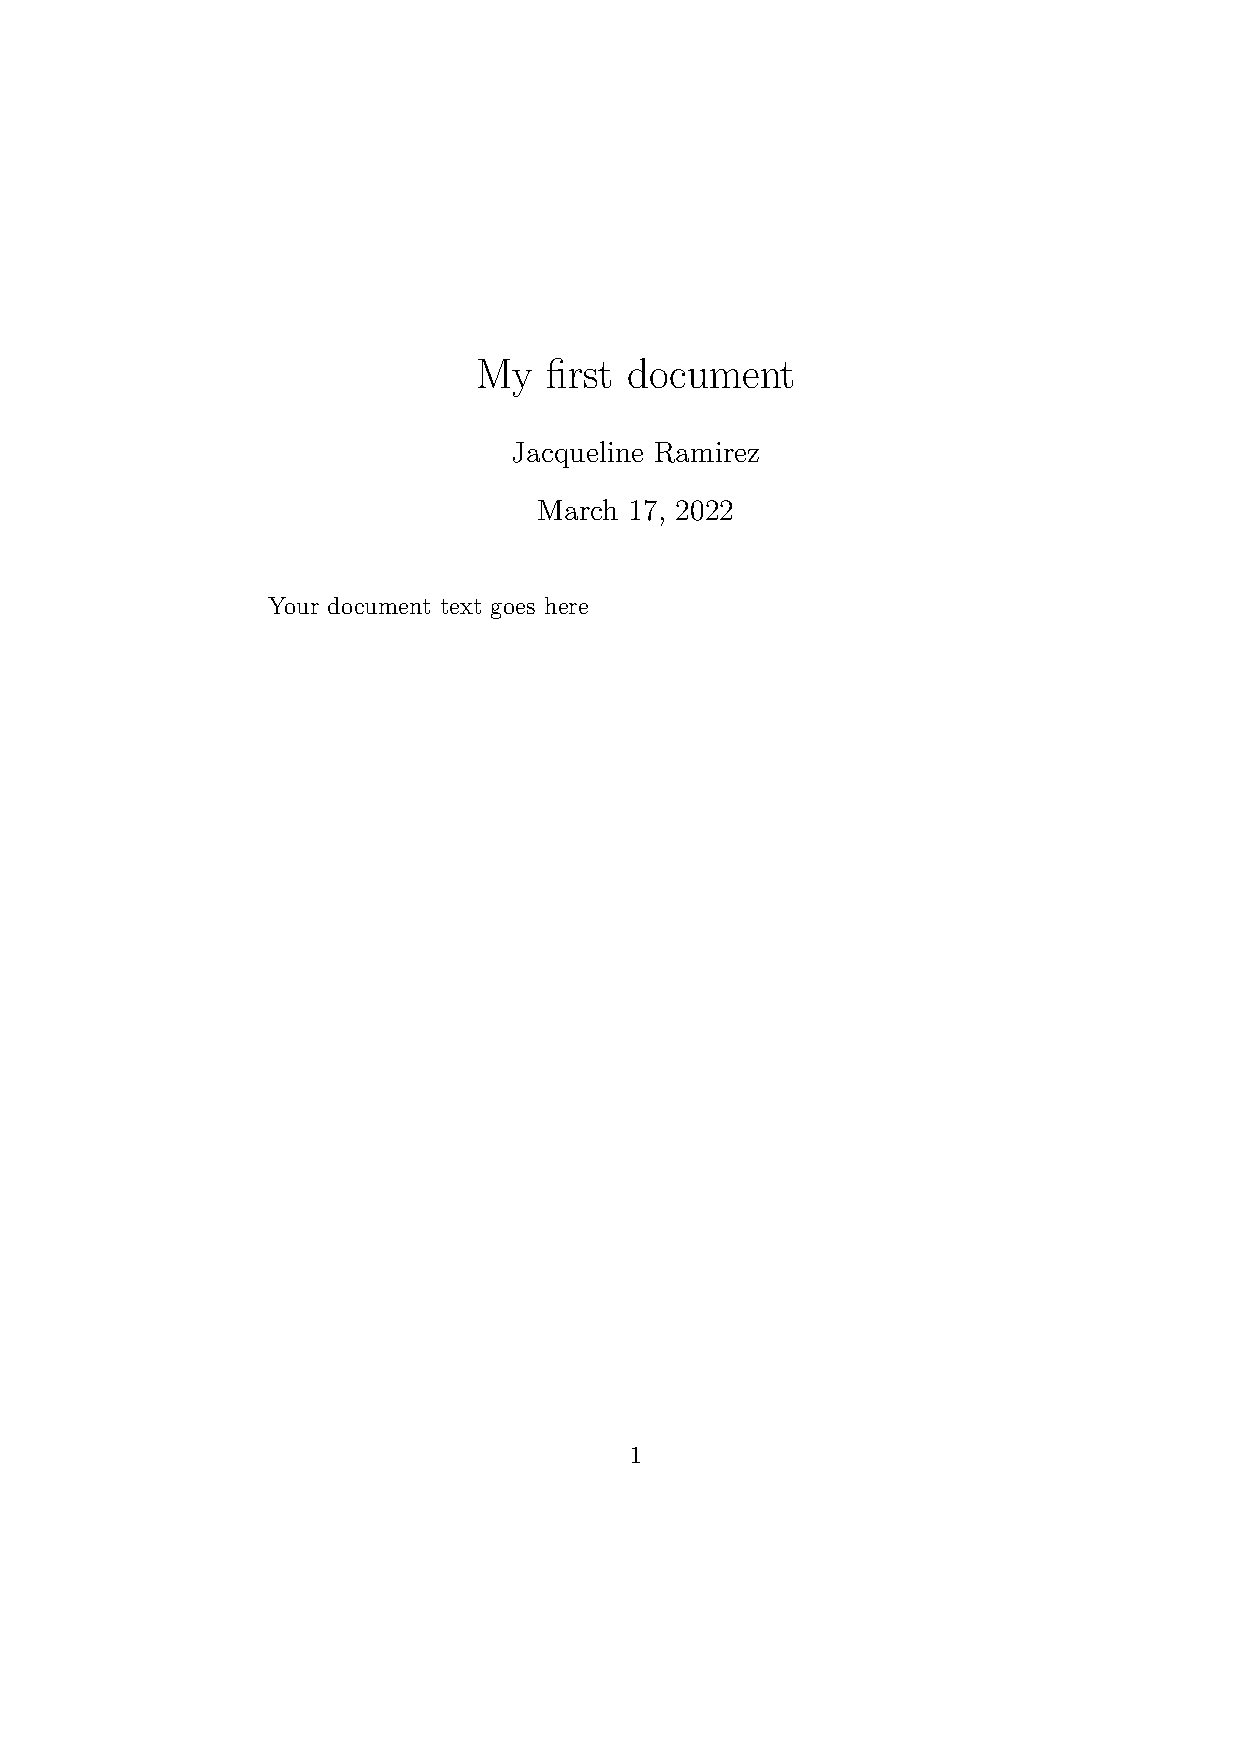
\includegraphics[width=10cm]{example/example.pdf}	}
	\end{figure}
\end{frame}

\section*{\LaTeX\ Examples}

\subsection*{Enumerate and Itemize}

\begin{frame}[fragile]{Enumerate}
	\begin{enumerate}
		\item For ordered lists
		\item Each item has a unique identifier
		\item [$\pi$.] Identifiers can be custom too!
	\end{enumerate}	
	\begin{lstlisting}[basicstyle=\small,]
\begin{enumerate}
	\item For ordered lists
	\item Each item has a unique identifier
	\item [$\pi$.] They can be custom too!
\end{enumerate}	
\end{lstlisting}
\end{frame}

\begin{frame}[fragile]{Itemize}
	\begin{itemize}
		\item For unordered lists
		\item No distinct order necessary
		\item You can nest Enumerate and Itemize!
			\begin{enumerate}
				\item [a.] This allows subitems
				\item [b.] You might need to specify identifiers 
			\end{enumerate}
	\end{itemize}	
	\begin{lstlisting}[basicstyle=\tiny]
\begin{itemize}
  \item For unordered lists
  \item No distinct order necessary
  \item You can nest Enumerate and Itemize!
	\begin{enumerate}
	  \item [a.] This allows subitems
	  \item [b.] You might need to specify identifiers 
	\end{enumerate}
\end{itemize}	
\end{lstlisting}
\end{frame}

\subsection*{Mathematics}

\begin{frame}[fragile]{Mathematics}
\LaTeX{} is great for typesetting mathematics. 
\[
	S_n = \frac{X_1 + X_2 + \cdots + X_n}{n}
	= \frac{1}{n}\sum_{i}^{n} X_i  
\]
\begin{lstlisting}
\LaTeX{} is great for typesetting mathematics.
\[
	S_n = \frac{X_1 + X_2 + \cdots + X_n}{n}
	= \frac{1}{n}\sum_{i}^{n} X_i  
\]
\end{lstlisting}
\end{frame}

\subsection*{Figures}
\begin{frame}[fragile]{Figures}
	\begin{figure}[H]
		\centering
		
\includegraphics[width=3cm]{figures/hkn.png}
		\caption{The HKN Logo}
		\label{fig:single}
	\end{figure}	
\begin{lstlisting}[basicstyle=\tiny]
\begin{figure}[H]
		\centering
		
\includegraphics[width=3cm]{figures/hkn.png}
		\caption{The HKN Logo}
		\label{fig:single}
\end{figure}
\end{lstlisting}
\end{frame}

\section*{Demo}
\subsection*{Overleaf Demo}
\begin{frame}{Overleaf Demo}
	\begin{itemize}
		\item Web based - no installation required
		\item Endorsed by Purdue with free Overleaf Professional
		\item Thousands of templates
		\item \href{https://www.overleaf.com/register}{https://www.overleaf.com/register}
	\end{itemize}	
\end{frame}

\subsection*{This presentation}
\begin{frame}{How was this presentation created?}
\begin{itemize}
	\item You guessed it! Using \LaTeX{}.
	\item Created using the \textbf{beamer} package and document class.
	\item One of thousands of \LaTeX{} packages.
	\item View on Overleaf \href{https://www.overleaf.com/read/zzjzcbpxpvsk}{https://www.overleaf.com/read/zzjzcbpxpvsk}
\end{itemize}	
\end{frame}

\subsection*{Conclusion}
\begin{frame}{Conclusion}
	\begin{itemize}
		\item Questions?
		\item Try it: \href{https://www.overleaf.com/register}{https://www.overleaf.com/register}
	\end{itemize}	
\end{frame}
\end{document}



